%==============================================================================
%  MATH 231 -- Linear Algebra I (Queens College, Fall 2026)
%  THE COMPLEX NUMBERS LECTURE
%
%  Lecture number not yet fixed -- this file is named by topic on purpose, since
%  the Lecture 1 material is expected to be split across several meetings.
%
%  AUDIENCE: this document is distributed to students.  Keep it free of
%  instructor-facing apparatus -- time budgets, pacing notes, teaching cues.
%  (The homework-review block that opens the meeting is scheduling, not
%  content, and deliberately does not appear here.)
%
%  CROSS-LECTURE DEPENDENCIES.  This lecture leans on the vectors lecture in
%  four places, each cross-referenced in the text:
%     - the norm of a 2-D vector          -> the modulus |z|
%     - <u,u> = ||u||^2                   -> z * conj(z) = |z|^2
%     - the orthogonality test <u,v> = 0  -> multiplication by i is a rotation
%     - the unit circle S^1               -> the complex numbers with |z| = 1
%
%  FOUR CORRECTIONS made against the drafted outline, all deliberate:
%   (a) conjugate is written \overline{z}, NOT \hat{z}.  The vectors lecture
%       already uses \hat{u} for a NORMALIZED vector; reusing the hat for
%       conjugation would collide inside the same course.
%   (b) i is defined by i^2 = -1, with "i = sqrt(-1)" given as the informal
%       reading.  Defining it as sqrt(-1) invites sqrt(-1)*sqrt(-1) = sqrt(1) = 1.
%   (c) division requires w != 0, i.e. c and d not BOTH zero.  The outline said
%       "at most one of the real numbers is 0", which is a different condition.
%   (d) Hamilton's carving is i^2 = j^2 = k^2 = ijk = -1; the outline dropped
%       the i^2 term.  Date: Monday 16 October 1843, Broome Bridge, Dublin.
%
%  Compile with pdflatex (standard TeX Live packages only; uses tikz).
%==============================================================================
\documentclass[11pt]{article}

\usepackage[margin=1in]{geometry}
\usepackage{amsmath,amssymb,amsthm}
\usepackage[dvipsnames]{xcolor}
\usepackage{enumitem}
\usepackage{booktabs}
\usepackage{array}
\usepackage[hidelinks]{hyperref}
\usepackage{titlesec}
\usepackage{needspace}
\usepackage{tikz}
\usetikzlibrary{arrows.meta}

%------------------------------------------------------------------ style ----
\titleformat{\section}{\large\bfseries\sffamily}{\thesection.}{0.6em}{}
\titleformat{\subsection}{\normalsize\bfseries\sffamily}{\thesubsection.}{0.5em}{}
\titlespacing*{\section}{0pt}{14pt}{6pt}

\theoremstyle{definition}
\newtheorem{defn}{Definition}
\newtheorem{ex}{Example}
\theoremstyle{remark}
\newtheorem*{rmk}{Remark}
\newtheorem*{hist}{Historical note}

\newcommand{\lookahead}{\par\smallskip\noindent
  \textbf{\sffamily\textcolor{RoyalBlue}{Looking ahead.}}\ \ignorespaces}
\newcommand{\lookback}{\par\smallskip\noindent
  \textbf{\sffamily\textcolor{ForestGreen}{Connection.}}\ \ignorespaces}

%--------------------------------------------------------------- notation ----
\newcommand{\R}{\mathbb{R}}
\newcommand{\C}{\mathbb{C}}
\newcommand{\Hq}{\mathbb{H}}
\newcommand{\Sph}[1]{\mathbb{S}^{#1}}
\newcommand{\vc}[1]{\mathbf{#1}}
\newcommand{\norm}[1]{\lVert #1\rVert}
\newcommand{\conj}[1]{\overline{#1}}
\newcommand{\Rez}{\operatorname{Re}}
\newcommand{\Imz}{\operatorname{Im}}

%------------------------------------------------------------- tikz helpers --
\tikzset{
  vecarr/.style   = {-{Stealth[length=2.6mm,width=2.0mm]},very thick},
  thinarr/.style  = {-{Stealth[length=2.2mm,width=1.7mm]},thick},
  axisline/.style = {->,gray!75,thin}
}
% \cplane{xmin}{xmax}{ymin}{ymax} -- a gridded complex plane
\newcommand{\cplane}[4]{%
  \draw[step=1cm,gray!25,very thin] (#1,#3) grid (#2,#4);
  \draw[axisline] (#1,0) -- (#2+0.55,0)
        node[right,font=\scriptsize,black]{$\Rez$};
  \draw[axisline] (0,#3) -- (0,#4+0.55)
        node[above,font=\scriptsize,black]{$\Imz$};
}
% \cpoint{x}{y}{colour}{label}{anchor}
\newcommand{\cpoint}[5]{%
  \fill[#3] (#1,#2) circle (2.1pt);
  \node[#5,font=\scriptsize,#3] at (#1,#2) {#4};
}

\title{\vspace{-1.2cm}\textbf{\sffamily MATH 231 -- Linear Algebra I}\\[4pt]
       {\large\sffamily Complex Numbers \textbullet\ and a First Look at
        Quaternions}\\[2pt]
       {\normalsize\sffamily Kiely Hall 326 \textbullet\
        Instructor: Kevin Bedoya}}
\author{}
\date{}

\begin{document}
\maketitle
\vspace{-1.6cm}

\noindent\textbf{What you should be able to do afterwards.} Explain why
$x^{2}+1$ has no real roots but two complex ones; write a complex number in the
form $a+bi$ and identify its real and imaginary parts; plot complex numbers on
the complex plane; add, subtract, multiply and divide them; take a conjugate and
say what it does geometrically; compute a modulus and use it to measure
distance; describe a disc by an inequality; write a point of the unit circle as
$\cos\theta+i\sin\theta$; state Euler's formula and Euler's identity; explain
why multiplying by $i$ is a rotation by $90^{\circ}$; state de Moivre's formula
and say what the roots of unity are; and describe what a quaternion is and where
quaternions are used.

\medskip
\noindent\textbf{Further reading.}
Axler, \emph{Linear Algebra Done Right}, Ch.~1 (the field $\C$) and Ch.~4
(polynomials, the fundamental theorem of algebra). Euler's formula, De~Moivre,
and quaternions are supplementary --- see the optional appendices.

%==============================================================================
\section{Where the real numbers run out}
%==============================================================================
Start with a polynomial you can already handle. Let
\[
  f(x)=x^{2}-1 .
\]
To find its roots, set $f(x)=0$: then $x^{2}=1$, so $x=\pm 1$. Two distinct
roots, both real, and the graph confirms them --- the parabola crosses the
$x$-axis at $-1$ and at $+1$.

Now change one sign. Let
\[
  f(x)=x^{2}+1 .
\]
The same procedure gives $x^{2}=-1$, so $x=\pm\sqrt{-1}$ --- and here the
procedure stops. There is no real number whose square is negative: squaring a
positive number gives a positive number, squaring a negative number also gives a
positive number, and $0^{2}=0$. So $\sqrt{-1}$ is undefined as a real quantity,
and the graph agrees: the parabola $y=x^{2}+1$ never touches the $x$-axis at
all.

\begin{center}
\begin{tikzpicture}[scale=0.8]
  \draw[axisline] (-2.5,0) -- (2.6,0) node[right,font=\scriptsize,black]{$x$};
  \draw[axisline] (0,-1.8) -- (0,5.2) node[above,font=\scriptsize,black]{$y$};
  \draw[BrickRed,thick,domain=-2.25:2.25,smooth,variable=\x]
        plot ({\x},{\x*\x-1});
  \fill (1,0) circle (2.1pt);
  \fill (-1,0) circle (2.1pt);
  \node[below right,font=\scriptsize] at (1.05,-0.06)  {$1$};
  \node[below left,font=\scriptsize]  at (-1.05,-0.06) {$-1$};
  \node[right,font=\scriptsize,BrickRed] at (2.05,3.7) {$y=x^{2}-1$};
  \node[font=\scriptsize] at (0,-2.5) {two real roots};
\end{tikzpicture}
\hspace{1.1cm}
\begin{tikzpicture}[scale=0.8]
  \draw[axisline] (-2.5,0) -- (2.6,0) node[right,font=\scriptsize,black]{$x$};
  \draw[axisline] (0,-1.8) -- (0,5.2) node[above,font=\scriptsize,black]{$y$};
  \draw[RoyalBlue,thick,domain=-2.0:2.0,smooth,variable=\x]
        plot ({\x},{\x*\x+1});
  \node[right,font=\scriptsize,RoyalBlue] at (1.9,4.5) {$y=x^{2}+1$};
  \node[font=\scriptsize] at (0,-2.5) {no real roots};
\end{tikzpicture}
\end{center}

\subsection*{Why the obstruction feels real}
There is a reason $\sqrt{-1}$ looks not merely difficult but \emph{meaningless}.
Think about what a square root measures. If a square has area $25$ square feet,
then $\sqrt{25}=5$ is the length of its side --- a positive quantity, because
lengths are positive. Ask for $\sqrt{-1}$ and you are asking for the side length
of a square whose area is $-1$ square foot. No such square exists: area cannot be
negative. The question has no answer because the question is malformed.

That was more or less the view for a long time. What changed was the discovery
that if you \emph{proceed anyway} --- carry the impossible quantity through the
computation and see what happens --- the answers that come out at the end are
correct, useful, and often real.

\begin{hist}
Square roots of negative numbers first forced themselves on
\textbf{Gerolamo Cardano} (Italian, 1501--1576) in his \emph{Ars Magna} of
\textbf{1545}, where they turned up while he was solving cubic equations.
Cardano did the arithmetic but distrusted it, calling such quantities useless.
It was \textbf{Rafael Bombelli} (Italian, 1526--1572) in his \emph{L'Algebra} of
\textbf{1572} who laid down consistent rules for calculating with them and
showed that they could be manipulated safely --- turning a curiosity into a
tool. The notation $i$ we use today was introduced much later, by
\textbf{Leonhard Euler} (Swiss, 1707--1783) in \textbf{1777}.
\end{hist}

%==============================================================================
\section{The imaginary unit, and complex numbers}
%==============================================================================
\begin{defn}[The imaginary unit]
The \textbf{imaginary unit} $i$ is the number defined by the property
\[
  i^{2}=-1 .
\]
It is informally written $i=\sqrt{-1}$, and read ``the square root of minus
one.''
\end{defn}

\begin{rmk}
Take $i^{2}=-1$ as the definition and treat $i=\sqrt{-1}$ as shorthand for it.
The radical notation is convenient but it invites a false move: the familiar
rule $\sqrt{a}\sqrt{b}=\sqrt{ab}$ is a theorem about \emph{non-negative} reals,
and applying it here would give the nonsense
$\sqrt{-1}\sqrt{-1}=\sqrt{1}=1$ instead of the correct $i^{2}=-1$. Work from
$i^{2}=-1$ and you will never trip over this.
\end{rmk}

\noindent With $i$ available, the polynomial that defeated us is solved. Since
$i^{2}=-1$ and $(-i)^{2}=(-1)^{2}i^{2}=i^{2}=-1$, both $i$ and $-i$ satisfy
$x^{2}=-1$. So
\[
  f(x)=x^{2}+1
  \qquad\text{has roots}\qquad
  x=\pm i .
\]
The graph told us the truth: $f$ has no \emph{real} roots. What it could not
show us is that $f$ has two \emph{imaginary} roots, because they do not live on
the $x$-axis. They live on a different line, in a plane we have not drawn yet.

\begin{defn}[Complex number]
A \textbf{complex number} is a number of the form
\[
  z = a + bi ,
  \qquad a,b\in\R ,
\]
and the set of all of them is denoted $\C$:
\[
  \C \;=\; \bigl\{\, a+bi \;:\; a,b\in\R \,\bigr\}.
\]
We write $z\in\C$. The real number $a$ is the \textbf{real part} of $z$ and the
real number $b$ is the \textbf{imaginary part}:
\[
  \Rez(z) := a,
  \qquad
  \Imz(z) := b .
\]
\end{defn}

\begin{rmk}
The imaginary part is the real number $b$, \emph{not} $bi$. For $z=3+2i$ we have
$\Rez(z)=3$ and $\Imz(z)=2$ --- both plain real numbers. Two complex numbers are
equal exactly when their real parts agree and their imaginary parts agree.
\end{rmk}

%==============================================================================
\section{The complex plane}
%==============================================================================
A complex number carries two independent real numbers, so it needs two axes to
be drawn. Geometrically, complex numbers are \textbf{points of a plane} --- the
\textbf{complex plane} --- laid out as follows:

\begin{itemize}[leftmargin=1.4em,itemsep=2pt]
  \item the horizontal axis carries the \emph{real} part, and is called the
        \textbf{real axis};
  \item the vertical axis carries the \emph{imaginary} part, and is called the
        \textbf{imaginary axis}.
\end{itemize}

\noindent So $z=a+bi$ is plotted at the point $(a,b)$.

Start with the two roots we just found. Both $i$ and $-i$ have real part $0$:
writing them out in full, $i=0+1i$ and $-i=0+(-1)i$, so
\[
  \Rez(i)=0,\quad \Imz(i)=1,
  \qquad\qquad
  \Rez(-i)=0,\quad \Imz(-i)=-1 .
\]
A real part of $0$ means no horizontal displacement, so both numbers sit
\emph{on} the imaginary axis --- one unit above the origin and one unit below.
This is the sense in which the roots of $x^{2}+1$ were invisible on our earlier
graph: they were never on the horizontal axis to begin with.

\begin{center}
% the two grids have different heights, so centre both on the text baseline
% rather than letting them sit bottom-aligned
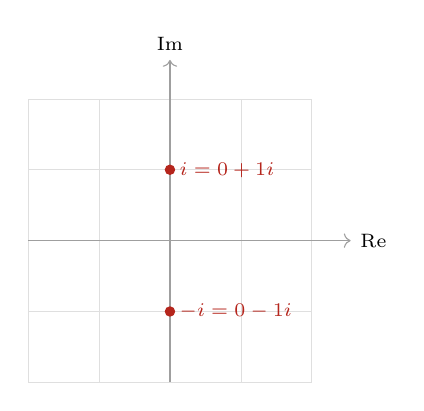
\begin{tikzpicture}[scale=0.9,baseline=(current bounding box.center)]
  \cplane{-2}{2}{-2}{2}
  \cpoint{0}{1}{BrickRed}{$i=0+1i$}{right}
  \cpoint{0}{-1}{BrickRed}{$-i=0-1i$}{right}
\end{tikzpicture}
\hspace{1.0cm}
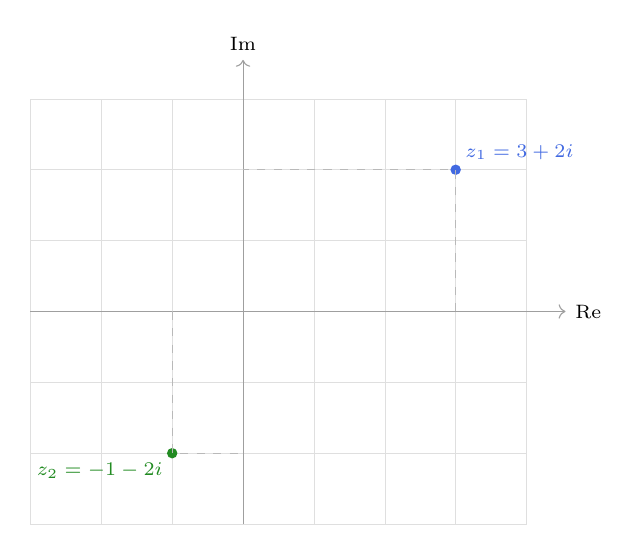
\begin{tikzpicture}[scale=0.9,baseline=(current bounding box.center)]
  \cplane{-3}{4}{-3}{3}
  \cpoint{3}{2}{RoyalBlue}{$z_1=3+2i$}{above right}
  \cpoint{-1}{-2}{ForestGreen}{$z_2=-1-2i$}{below left}
  \draw[gray!55,dashed] (3,0) -- (3,2) -- (0,2);
  \draw[gray!55,dashed] (-1,0) -- (-1,-2) -- (0,-2);
\end{tikzpicture}
\end{center}

\noindent In the right-hand picture the dashed lines read off the two parts:
$z_1=3+2i$ sits $3$ to the right and $2$ up, while $z_2=-1-2i$ sits $1$ to the
left and $2$ down.

%------------------------------------------------------------------------------
\subsection{Every real number is a complex number}
%------------------------------------------------------------------------------
What is a complex number with imaginary part $0$? It is $z=a+0i=a$ --- an
ordinary real number, sitting on the real axis. So the real numbers are not a
separate species; they are exactly the complex numbers whose imaginary part
vanishes. Every real number is a complex number, which is to say
\[
  \R \subset \C .
\]
The real line is the horizontal axis of the complex plane, and $\C$ is what you
get by allowing motion off that line.

%------------------------------------------------------------------------------
\subsection{Complex numbers are two-dimensional}
%------------------------------------------------------------------------------
The real numbers form a line: one number pins down a position, so $\R$ is
one-dimensional. A complex number needs \emph{two} real numbers, chosen
independently, to pin down its position in the plane --- two degrees of freedom.
So $\C$ is two-dimensional.

\lookback This is the same counting we used for $\R^{2}$ in the vectors lecture,
and the resemblance is not a coincidence. A complex number $a+bi$ and a vector
$[\,a,\,b\,]$ carry identical data. Accordingly, several operations on complex
numbers are performed \emph{componentwise}, exactly as with vectors, and for
those operations the two objects are genuinely interchangeable.

\lookahead Where they stop being interchangeable is multiplication. There is no
useful way to multiply two vectors in $\R^{2}$ and get a third vector --- but
complex numbers multiply, and divide, perfectly well. That extra structure is
the whole reason $\C$ deserves its own name, and it is what makes the rotation
results of \S7 possible.

%==============================================================================
\section{Arithmetic}
%==============================================================================
%------------------------------------------------------------------------------
\subsection{Addition and subtraction}
%------------------------------------------------------------------------------
Collect real parts with real parts and imaginary parts with imaginary parts.

\begin{defn}[Addition and subtraction in $\C$]
For $z=a+bi$ and $w=c+di$ in $\C$,
\[
  z+w = (a+c)+(b+d)i,
  \qquad
  z-w = (a-c)+(b-d)i .
\]
\end{defn}

\noindent Both are componentwise, and both return a complex number --- so $\C$
is closed under addition and subtraction.

\begin{ex}
$(3+2i)+(1+4i) = (3+1)+(2+4)i = 4+6i$.
\end{ex}

\begin{ex}
$(5-3i)-(2+i) = (5-2)+(-3-1)i = 3-4i$.
\end{ex}

\begin{ex}
$(-2+5i)+(6-5i) = (-2+6)+(5-5)i = 4+0i = 4$. \\
Worth noticing: the sum of two numbers that are \emph{not} real can be real. The
imaginary parts cancelled.
\end{ex}

%------------------------------------------------------------------------------
\subsection{Multiplication}
%------------------------------------------------------------------------------
Multiplication needs no new rule at all. Expand the product as you would any two
binomials, and then use $i^{2}=-1$ to clean up:
\[
  (a+bi)(c+di)
  = ac + adi + bci + bd\,i^{2}
  = ac + adi + bci - bd ,
\]
and collecting the parts,
\[
  \boxed{\;(a+bi)(c+di) = (ac-bd) + (ad+bc)\,i\;}
\]
The single step that does all the work is $bd\,i^{2}=-bd$: a term that started
out imaginary lands in the real part, with its sign flipped.

\begin{ex}
$(3+2i)(1+4i) = 3 + 12i + 2i + 8i^{2} = 3 + 14i - 8 = -5 + 14i$.
\end{ex}

\begin{ex}
$(2+3i)(2-3i) = 4 - 6i + 6i - 9i^{2} = 4 + 9 = 13$. \\
The imaginary parts cancelled and $i^{2}$ turned $-9i^{2}$ into $+9$, leaving a
real answer. This is not an accident, and \S4.3 explains it.
\end{ex}

\begin{rmk}
Multiplication is emphatically \emph{not} componentwise: the real part of the
product mixes $a$, $b$, $c$ and $d$ together. Compare addition, where the first
slots never talk to the second. This is precisely the point at which a complex
number stops behaving like a vector in $\R^{2}$.
\end{rmk}

%------------------------------------------------------------------------------
\subsection{The conjugate}
%------------------------------------------------------------------------------
\begin{defn}[Complex conjugate]
The \textbf{conjugate} of $z=a+bi$ is
\[
  \conj{z} = a-bi ,
\]
obtained by flipping the sign of the imaginary part. It is read ``$z$-bar.''
\end{defn}

\begin{rmk}
Some texts write $z^{*}$ for the conjugate. We use the overline
$\conj{z}$ throughout, and we specifically avoid the hat: in the vectors lecture
$\hat{\vc{u}}$ already means the \emph{normalization} of $\vc{u}$, and reusing
the hat here would collide.
\end{rmk}

\noindent Geometrically, conjugation is a \textbf{reflection about the real
axis}. The real part is untouched, so the horizontal position stays; the
imaginary part changes sign, so the point flips to the other side of the
horizontal axis. It is the mirror image of $z$ in the real axis.

\begin{center}
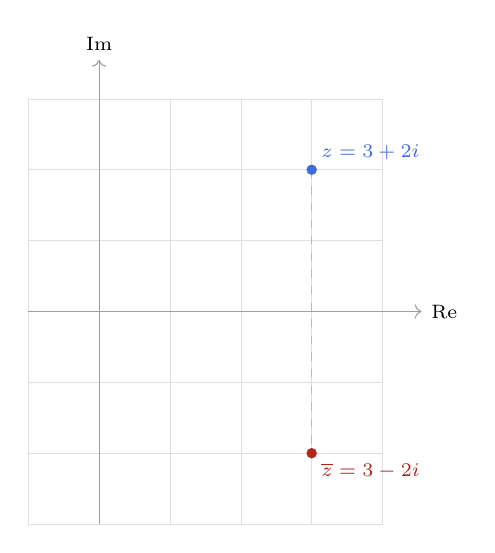
\begin{tikzpicture}[scale=0.9]
  \cplane{-1}{4}{-3}{3}
  \draw[gray!55,dashed] (3,2) -- (3,-2);
  \cpoint{3}{2}{RoyalBlue}{$z=3+2i$}{above right}
  \cpoint{3}{-2}{BrickRed}{$\conj{z}=3-2i$}{below right}
\end{tikzpicture}
\end{center}

\noindent Two facts about conjugation that we will use immediately. First, a
number equals its own conjugate exactly when $b=0$, that is, exactly when it is
real. Second, and this is the useful one:
\[
  z\conj{z} = (a+bi)(a-bi) = a^{2} - abi + abi - b^{2}i^{2} = a^{2}+b^{2} .
\]
So $z\conj{z}$ is always a \emph{real}, non-negative number --- the imaginary
parts cancel by construction. That is what happened in the second multiplication
example above, where $(2+3i)(2-3i)=13$.

%------------------------------------------------------------------------------
\subsection{Division}
%------------------------------------------------------------------------------
Division is possible in $\C$ too, provided the denominator is not zero. The
obstacle is cosmetic: a quotient like $(3+2i)/(1-i)$ is a perfectly good complex
number, but it is not yet written in the form $a+bi$, so we cannot read off its
real and imaginary parts.

The trick is the previous subsection. We want a \emph{real} denominator, and
$w\conj{w}$ is always real --- so multiply the numerator and the denominator by
the conjugate of the denominator.

\begin{quote}
\textbf{To divide.} Let $z=a+bi$ and $w=c+di$ with $w\neq 0$ (that is, $c$ and
$d$ not both zero). Then
\[
  \frac{z}{w}
  = \frac{z}{w}\cdot\frac{\conj{w}}{\conj{w}}
  = \frac{(a+bi)(c-di)}{(c+di)(c-di)}
  = \frac{(ac+bd)+(bc-ad)i}{c^{2}+d^{2}}
  = \frac{ac+bd}{c^{2}+d^{2}} + \frac{bc-ad}{c^{2}+d^{2}}\,i .
\]
\end{quote}

\noindent Since $w\neq0$ we have $c^{2}+d^{2}>0$, so the two fractions are
honest real numbers and the result is in the form $a+bi$. Note that multiplying
by $\conj{w}/\conj{w}$ multiplies by $1$: the value is unchanged, only its
appearance.

\begin{ex}[A division, worked out]
Compute $\dfrac{3+2i}{1-i}$.

The denominator is $w=1-i$, so $\conj{w}=1+i$. Multiply top and bottom by it:
\[
  \frac{3+2i}{1-i}
  = \frac{3+2i}{1-i}\cdot\frac{1+i}{1+i}
  = \frac{(3+2i)(1+i)}{(1-i)(1+i)} .
\]
Numerator: $(3+2i)(1+i) = 3+3i+2i+2i^{2} = 3+5i-2 = 1+5i$. \\
Denominator: $(1-i)(1+i) = 1+i-i-i^{2} = 1+1 = 2$. \\
Therefore
\[
  \frac{3+2i}{1-i} = \frac{1+5i}{2} = \frac{1}{2}+\frac{5}{2}\,i ,
\]
which is in the form $a+bi$ with $a=\tfrac12$ and $b=\tfrac52$.
\end{ex}

\begin{rmk}
So $\C$ supports addition, subtraction, multiplication, and division by anything
nonzero. A number system with all four is called a \emph{field}, and $\C$ is one
--- just as $\R$ is. This is why complex scalars can be used anywhere real
scalars can, a fact we will lean on when eigenvalues turn out to be complex.
\end{rmk}

%==============================================================================
\section{The modulus, distance, and discs}
%==============================================================================
%------------------------------------------------------------------------------
\subsection{From absolute value to modulus}
%------------------------------------------------------------------------------
For a real number $x$, the absolute value $\lvert x\rvert$ measures the distance
from $x$ to $0$, and $\lvert x-a\rvert$ measures the distance from $x$ to $a$.
That works because the real numbers lie on a \emph{line}: there is only one
direction to travel, so a single subtraction and a sign-strip is enough.

Complex numbers live on a plane, so distance needs the two-dimensional
measurement instead.

\begin{defn}[Modulus]
The \textbf{modulus} of $z=a+bi$ is
\[
  \lvert z\rvert = \sqrt{a^{2}+b^{2}} ,
\]
the Euclidean distance from $z$ to the origin of the complex plane.
\end{defn}

\lookback This is the norm of the vector $[\,a,\,b\,]$ from the vectors lecture,
under a different name and the same Pythagoras: the horizontal leg has length
$\lvert a\rvert$, the vertical leg $\lvert b\rvert$, and $\lvert z\rvert$ is the
hypotenuse. The identity $z\conj{z}=a^{2}+b^{2}$ of \S4.3 can therefore be
restated as
\[
  \lvert z\rvert^{2} = z\conj{z} ,
\]
which is the exact counterpart of $\langle \vc{u},\vc{u}\rangle=\norm{\vc{u}}^{2}$.
Conjugation plays the role that the second copy of the vector played in the dot
product.

\begin{center}
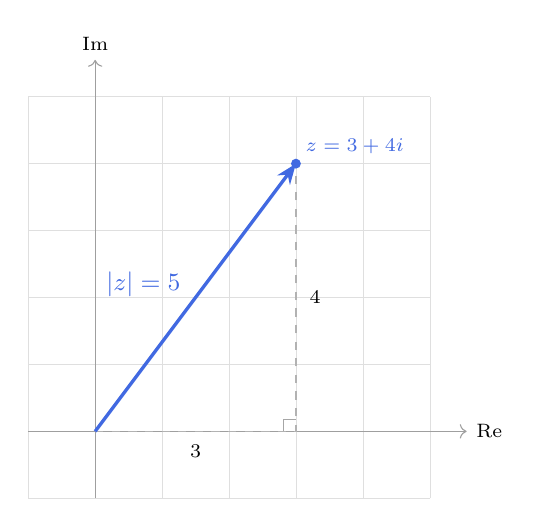
\begin{tikzpicture}[scale=0.85]
  \cplane{-1}{5}{-1}{5}
  \draw[gray!60,dashed] (0,0) -- (3,0) -- (3,4);
  \draw[gray!70] (2.82,0) -- (2.82,0.18) -- (3,0.18);
  \draw[vecarr,RoyalBlue] (0,0) -- (3,4);
  \cpoint{3}{4}{RoyalBlue}{$z=3+4i$}{above right}
  \node[below,font=\scriptsize] at (1.5,-0.06) {$3$};
  \node[right,font=\scriptsize] at (3.06,2)    {$4$};
  \node[left,font=\small,RoyalBlue] at (1.42,2.2) {$\lvert z\rvert=5$};
\end{tikzpicture}
\end{center}

\begin{ex}
$\lvert 3+4i\rvert=\sqrt{9+16}=\sqrt{25}=5$.
\end{ex}

\begin{ex}
$\lvert -1+i\rvert=\sqrt{(-1)^{2}+1^{2}}=\sqrt{2}$.
\end{ex}

\begin{ex}
$\lvert i\rvert=\sqrt{0^{2}+1^{2}}=1$, and likewise $\lvert -i\rvert=1$. The two
roots of $x^{2}+1$ both sit at distance $1$ from the origin.
\end{ex}

%------------------------------------------------------------------------------
\subsection{Distance between two complex numbers}
%------------------------------------------------------------------------------
The modulus also measures distances between points, exactly as absolute value
does on the line: for $z,w\in\C$,
\[
  \lvert z-w\rvert
  \;=\;\text{the distance from } z \text{ to } w .
\]
Subtract to get the displacement between them, then take its modulus to get the
displacement's length. The order does not matter, since $\lvert z-w\rvert
=\lvert w-z\rvert$.

\begin{ex}
The distance from $z=3+2i$ to $w=1-i$ is
\[
  \lvert z-w\rvert = \lvert (3-1)+(2-(-1))i\rvert = \lvert 2+3i\rvert
  = \sqrt{4+9} = \sqrt{13}.
\]
\end{ex}

%------------------------------------------------------------------------------
\subsection{Discs}
%------------------------------------------------------------------------------
Once distance is available, whole \emph{regions} of the complex plane can be
described by a single inequality. The most common such regions in mathematics
are \textbf{discs}.

\begin{itemize}[leftmargin=1.4em,itemsep=4pt]
  \item $\lvert z\rvert\le 1$ is the set of complex numbers at distance at most
        $1$ from the origin: the \textbf{disc of radius $1$ centred at the
        origin}, boundary included. It is called the \emph{closed unit disc}.
  \item $\lvert z-w\rvert\le 2$ with $w=1+2i$ is the set of complex numbers at
        distance at most $2$ from the point $1+2i$: the \textbf{disc of radius
        $2$ centred at $1+2i$}.
\end{itemize}

\noindent The pattern generalises: $\lvert z-w\rvert\le r$ is the disc of radius
$r$ centred at $w$. Replacing $\le$ by $<$ removes the boundary circle, and
replacing it by $=$ leaves the boundary circle alone.

\begin{center}
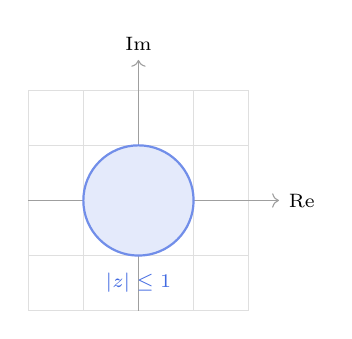
\begin{tikzpicture}[scale=0.7,baseline=(current bounding box.center)]
  \cplane{-2}{2}{-2}{2}
  \fill[RoyalBlue!14] (0,0) circle (1);
  \draw[RoyalBlue!75,thick] (0,0) circle (1);
  \node[font=\scriptsize,RoyalBlue] at (0,-1.5) {$\lvert z\rvert\le 1$};
\end{tikzpicture}
\hspace{1.4cm}
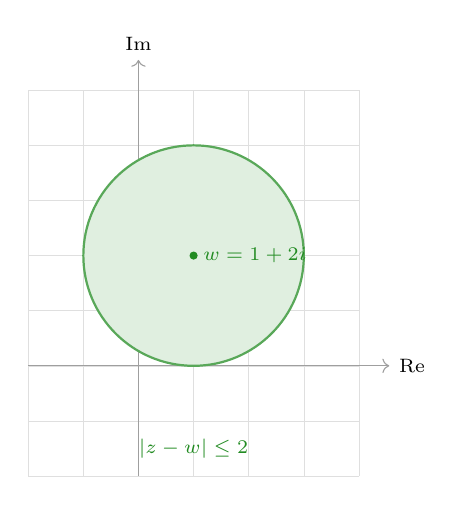
\begin{tikzpicture}[scale=0.7,baseline=(current bounding box.center)]
  \cplane{-2}{4}{-2}{5}
  \fill[ForestGreen!14] (1,2) circle (2);
  \draw[ForestGreen!75,thick] (1,2) circle (2);
  \cpoint{1}{2}{ForestGreen}{$w=1+2i$}{right}
  \node[font=\scriptsize,ForestGreen] at (1,-1.5) {$\lvert z-w\rvert\le 2$};
\end{tikzpicture}
\end{center}

%==============================================================================
\section{The unit circle and Euler's formula}
%==============================================================================
Narrow attention to the complex numbers of modulus exactly $1$:
\[
  \lvert z\rvert = 1 .
\]
By the previous section this is a circle of radius $1$ centred at the origin ---
the \textbf{unit circle} of the complex plane.

\lookback This is the same set, drawn in the same place, as the unit vectors
$\Sph{1}$ of the vectors lecture: $\lvert z\rvert=1$ is $a^{2}+b^{2}=1$, which
is what $\norm{\vc{u}}=1$ was. The complex numbers of unit modulus \emph{are}
the unit vectors, now equipped with the ability to multiply one another.

%------------------------------------------------------------------------------
\subsection{Trigonometric form}
%------------------------------------------------------------------------------
Take a point $z=a+bi$ on the unit circle and drop a perpendicular from it to the
real axis. This produces a right triangle whose hypotenuse runs from the origin
to $z$ and therefore has length $\lvert z\rvert=1$. Call $\theta$ the angle at
the origin, measured from the positive real axis up to the hypotenuse.

% keep the derivation, the boxed result, and the figure that shows them together
\Needspace*{22\baselineskip}
Now read off the two legs by trigonometry. The horizontal leg is adjacent to
$\theta$ and the vertical leg is opposite it, and the hypotenuse is $1$, so
\[
  \cos\theta = \frac{a}{1} = a,
  \qquad
  \sin\theta = \frac{b}{1} = b .
\]
The two parts of $z$ \emph{are} the cosine and the sine:
\[
  \boxed{\;z = \cos\theta + i\sin\theta\;}
\]

\begin{center}
\begin{tikzpicture}[scale=1.9]
  \draw[axisline] (-1.35,0) -- (1.6,0) node[right,font=\scriptsize,black]{$\Rez$};
  \draw[axisline] (0,-1.35) -- (0,1.6) node[above,font=\scriptsize,black]{$\Imz$};
  \draw[gray!55] (0,0) circle (1);
  \draw[gray!60,dashed] (0.6,0.8) -- (0.6,0);
  \draw[gray!70] (0.53,0) -- (0.53,0.07) -- (0.6,0.07);
  \draw[vecarr,RoyalBlue] (0,0) -- (0.6,0.8);
  \draw[gray!80,thin] (0:0.3) arc (0:53.13:0.3);
  \node[font=\scriptsize] at (26:0.42) {$\theta$};
  \cpoint{0.6}{0.8}{RoyalBlue}{$z$}{above right}
  \node[below,font=\scriptsize] at (0.3,-0.04)  {$a=\cos\theta$};
  \node[right,font=\scriptsize] at (0.64,0.42)  {$b=\sin\theta$};
  \node[above left,font=\scriptsize,RoyalBlue] at (0.33,0.47) {$1$};
\end{tikzpicture}
\end{center}

\noindent Notice what has happened to the number of variables. A general complex
number needed two real numbers. A complex number \emph{on the unit circle} needs
only one, namely $\theta$: the modulus is already fixed at $1$, so only the
angle is free. So $z$ has become a function of $\theta$, and varying $\theta$
walks $z$ around the circle --- once around for every increase of $2\pi$.

%------------------------------------------------------------------------------
\subsection{Euler's formula}
%------------------------------------------------------------------------------
That combination of cosine and sine has a startling second description.

\begin{quote}
\textbf{Euler's formula.} For every real $\theta$,
\[
  e^{i\theta} = \cos\theta + i\sin\theta ,
\]
where $e^{x}=\exp(x)$ is the ordinary exponential function.
\end{quote}

\noindent Understanding \emph{why} an exponential should equal a combination of
trigonometric functions is beyond what we need today. If you would like to see
it, Appendix~A derives the formula from scratch using the Maclaurin series of
$e^{x}$, $\cos x$ and $\sin x$; the derivation is short and genuinely one of the
most satisfying calculations in mathematics.

For now, take Euler's formula as a licence to write any point of the unit circle
as a single exponential. It immediately yields the most quoted equation in the
subject. Put $\theta=\pi$:
\[
  e^{i\pi} = \cos\pi + i\sin\pi = -1 + 0i = -1 ,
\]
which is usually written

\begin{quote}
\textbf{Euler's identity.}
\[
  e^{i\pi} + 1 = 0 .
\]
\end{quote}

\noindent Five of the most important constants in mathematics --- $e$, $i$,
$\pi$, $1$ and $0$ --- tied together by one equation containing nothing else.

%==============================================================================
\section{Multiplying by $i$ is a rotation}
%==============================================================================
Here is the property that makes complex numbers indispensable in applications.
We will find it first by experiment and then prove it.

Start with $z=1$. Written in full that is $1+0i$, so $a=1$ and $b=0$, and
$\lvert z\rvert=\sqrt{1+0}=1$ --- it is on the unit circle. Now multiply
repeatedly by $i$ and watch where the point goes:
\[
  1
  \;\xrightarrow{\;\times i\;}\;
  i
  \;\xrightarrow{\;\times i\;}\;
  i^{2}=-1
  \;\xrightarrow{\;\times i\;}\;
  -i
  \;\xrightarrow{\;\times i\;}\;
  -i^{2}=1 .
\]
Each step turns the point through a quarter turn counter-clockwise, and four
steps return it to where it began.

\begin{center}
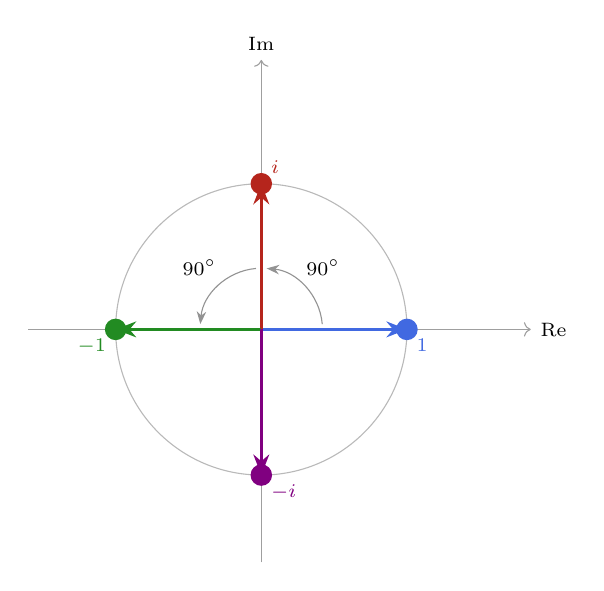
\begin{tikzpicture}[scale=1.85]
  \draw[axisline] (-1.6,0) -- (1.85,0) node[right,font=\scriptsize,black]{$\Rez$};
  \draw[axisline] (0,-1.6) -- (0,1.85) node[above,font=\scriptsize,black]{$\Imz$};
  \draw[gray!55] (0,0) circle (1);
  \draw[vecarr,RoyalBlue]   (0,0) -- (1,0);
  \draw[vecarr,BrickRed]    (0,0) -- (0,1);
  \draw[vecarr,ForestGreen] (0,0) -- (-1,0);
  \draw[vecarr,Purple]      (0,0) -- (0,-1);
  \draw[gray!85,thin,-{Stealth[length=1.6mm]}] (5:0.42) arc (5:85:0.42);
  \node[font=\scriptsize] at (45:0.60) {$90^{\circ}$};
  \draw[gray!85,thin,-{Stealth[length=1.6mm]}] (95:0.42) arc (95:175:0.42);
  \node[font=\scriptsize] at (135:0.60) {$90^{\circ}$};
  \cpoint{1}{0}{RoyalBlue}{$1$}{below right}
  \cpoint{0}{1}{BrickRed}{$i$}{above right}
  \cpoint{-1}{0}{ForestGreen}{$-1$}{below left}
  \cpoint{0}{-1}{Purple}{$-i$}{below right}
\end{tikzpicture}
\end{center}

\subsection*{Proving the angle is exactly $90^{\circ}$}
Experiment is not proof, and we have the tools to settle it. Take an arbitrary
complex number $z=a+bi$ and multiply by $i$:
\[
  w = (a+bi)\,i = ai + bi^{2} = -b + ai .
\]
Now hand both numbers to the vectors lecture. As vectors,
\[
  z \;\longleftrightarrow\; \vc{z}=[\,a,\,b\,],
  \qquad
  w \;\longleftrightarrow\; \vc{w}=[\,-b,\,a\,],
\]
and their dot product is
\[
  \langle \vc{z},\vc{w}\rangle
  = a(-b) + b(a)
  = -ab + ab
  = 0 .
\]
By the orthogonality test, a dot product of zero means the two are orthogonal
--- so $z$ and $iz$ meet at a right angle, for \emph{every} $z$. That is the
$90^{\circ}$ claim, proved in three lines.

One detail finishes the job. Orthogonality alone would permit the length to
change as well; but
\[
  \lvert w\rvert = \sqrt{(-b)^{2}+a^{2}} = \sqrt{a^{2}+b^{2}} = \lvert z\rvert ,
\]
so multiplication by $i$ preserves the modulus. Same distance from the origin,
turned through a right angle: that is a \emph{rotation}, not a rotation combined
with a stretch.

\begin{quote}
\textbf{Multiplication by $i$} rotates a complex number by $90^{\circ}$
\textbf{counter-clockwise} about the origin.
\end{quote}

\noindent And the mirror statement holds too. Multiplying by $-i$ gives
$(a+bi)(-i) = -ai - bi^{2} = b - ai$, i.e.\ the vector $[\,b,\,-a\,]$, whose dot
product with $[\,a,\,b\,]$ is $ab-ba=0$ --- again orthogonal, again the same
modulus, but the turn goes the other way:

\begin{quote}
\textbf{Multiplication by $-i$} rotates a complex number by $90^{\circ}$
\textbf{clockwise} about the origin.
\end{quote}

\lookahead A quarter turn is the special case $\theta=\pi/2$ of something much
more general. Since $i=e^{i\pi/2}$ by Euler's formula, multiplying by $i$ is
multiplying by $e^{i\pi/2}$; and multiplying by $e^{i\theta}$ turns out to
rotate by $\theta$, for any angle at all. \S8 puts that to work.

%==============================================================================
\section{De Moivre's formula, the roots of unity, and how many roots there are}
%==============================================================================
%------------------------------------------------------------------------------
\subsection{De Moivre's formula}
%------------------------------------------------------------------------------
Return to Euler's formula, and rename the variable $x$ to emphasise that it need
not be thought of as an angle on a particular picture:
\[
  e^{ix} = \cos x + i\sin x .
\]
This function is sometimes written $\operatorname{cis}(x)$ --- ``cosine plus
$i$ sine'' --- which is a useful abbreviation to recognise.

Now raise both sides to an integer power $n$:
\[
  \bigl(e^{ix}\bigr)^{n} = \bigl(\cos x + i\sin x\bigr)^{n} .
\]
The left side simplifies by the ordinary law of exponents,
$\bigl(e^{ix}\bigr)^{n}=e^{ixn}$. And $e^{ixn}$ is just Euler's formula again,
read with $xn$ in place of $x$:
\[
  e^{i(xn)} = \cos(xn) + i\sin(xn) .
\]
Comparing the two expressions for the same quantity gives:

\begin{quote}
\textbf{De Moivre's formula.} For every real $x$ and every integer $n$,
\[
  \bigl(\cos x + i\sin x\bigr)^{n} = \cos(nx) + i\sin(nx) .
\]
\end{quote}

\noindent Read it as a statement about work saved. The left-hand side asks you
to multiply out an $n$-th power of a binomial; the right-hand side says the
answer is obtained by simply \emph{multiplying the angle by $n$}. Raising to a
power on the unit circle is nothing more than scaling an angle.

%------------------------------------------------------------------------------
\subsection{The roots of unity}
%------------------------------------------------------------------------------
De Moivre's formula makes short work of a classical question.

\begin{quote}
The \textbf{$n$-th roots of unity} are the complex numbers that give $1$ when
raised to the $n$-th power --- the solutions of $z^{n}=1$.
\end{quote}

\noindent Over the real numbers this question is dull: $z^{2}=1$ has the two
solutions $\pm1$, and $z^{3}=1$ has only $z=1$. Over the complex numbers it is
beautiful. There are always exactly $n$ solutions, and de Moivre says where:
taking $z=\cos\theta+i\sin\theta$ on the unit circle, $z^{n}=1$ requires
$\cos(n\theta)+i\sin(n\theta)=1$, which happens exactly when $n\theta$ is a
whole number of full turns. So $\theta=2\pi k/n$ for $k=0,1,\dots,n-1$, giving
\[
  z_k = \cos\frac{2\pi k}{n} + i\sin\frac{2\pi k}{n} = e^{2\pi i k/n}.
\]
Geometrically the answer is as clean as it could be: the $n$ roots are spaced
evenly around the unit circle, one of them always at $1$, and joining them up
produces a regular $n$-gon.

\begin{ex}[The fourth roots of unity]
For $n=4$ the roots are $1$, $i$, $-1$, $-i$ --- exactly the four points we
cycled through in \S6 by repeatedly multiplying by $i$. They form a square.
Indeed $i^{4}=(i^{2})^{2}=(-1)^{2}=1$, as required.
\end{ex}

\begin{center}
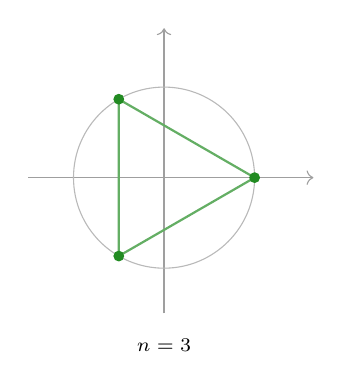
\begin{tikzpicture}[scale=1.15]
  \draw[axisline] (-1.5,0) -- (1.65,0);
  \draw[axisline] (0,-1.5) -- (0,1.65);
  \draw[gray!55] (0,0) circle (1);
  \draw[ForestGreen!70,thick] (0:1) -- (120:1) -- (240:1) -- cycle;
  \foreach \a in {0,120,240} { \fill[ForestGreen] (\a:1) circle (1.7pt); }
  \node[font=\scriptsize] at (0,-1.85) {$n=3$};
\end{tikzpicture}
\hspace{1.2cm}
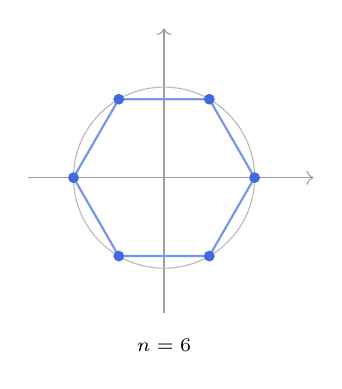
\begin{tikzpicture}[scale=1.15]
  \draw[axisline] (-1.5,0) -- (1.65,0);
  \draw[axisline] (0,-1.5) -- (0,1.65);
  \draw[gray!55] (0,0) circle (1);
  \draw[RoyalBlue!70,thick] (0:1) -- (60:1) -- (120:1) -- (180:1)
                            -- (240:1) -- (300:1) -- cycle;
  \foreach \a in {0,60,120,180,240,300} { \fill[RoyalBlue] (\a:1) circle (1.7pt); }
  \node[font=\scriptsize] at (0,-1.85) {$n=6$};
\end{tikzpicture}
\end{center}

%------------------------------------------------------------------------------
\subsection{How many roots does a polynomial have?}
%------------------------------------------------------------------------------
We opened this lecture with a polynomial that had two real roots and one that
had none. Over $\C$ that irregularity disappears entirely.

\begin{quote}
\textbf{Fundamental theorem of algebra} (also called \emph{d'Alembert's
theorem}). Every non-constant polynomial with complex coefficients has at least
one complex root. Consequently a polynomial of degree $n$ has exactly $n$
complex roots, counted with multiplicity.
\end{quote}

\noindent In plain terms: once you allow complex numbers, \emph{every}
polynomial factors completely, and the number of roots is simply the degree ---
no exceptions, no special cases. Our two opening examples both have degree $2$
and therefore both have exactly two roots. For $x^{2}-1$ they are $\pm1$ and
happen to be real; for $x^{2}+1$ they are $\pm i$ and are not. Nothing was ever
missing from $x^{2}+1$; we were simply looking in a space that was too small.

\begin{hist}
The result is named for \textbf{Jean-Baptiste le Rond d'Alembert}, who attempted
a proof in 1746, though the first substantially complete proof is due to
\textbf{Carl Friedrich Gauss} in 1799. Despite the name, every known proof uses
tools from analysis or topology rather than algebra alone.
\end{hist}

%==============================================================================
\section{Where this gets used}
%==============================================================================
The rotation property of \S6 is not a curiosity; it is the reason complex
numbers appear in engineering and computer graphics.

\subsubsection*{Rotating things in two dimensions}
Suppose you want to rotate a point of the plane through an angle $\theta$ about
the origin --- a sprite in a game, an image in an editor, a robot's heading.
Encode the point $(x,y)$ as the complex number $z=x+iy$ and multiply by
$e^{i\theta}$:
\[
  z\,e^{i\theta}
  = (x+iy)(\cos\theta+i\sin\theta)
  = \bigl(x\cos\theta - y\sin\theta\bigr)
    + i\bigl(x\sin\theta + y\cos\theta\bigr).
\]
Reading off the two parts, the rotated point is
$(x\cos\theta-y\sin\theta,\;x\sin\theta+y\cos\theta)$. A rotation of the plane
has become a \emph{single multiplication}. Composing two rotations is then just
$e^{i\alpha}e^{i\beta}=e^{i(\alpha+\beta)}$ --- angles add, which is exactly what
rotations should do.

\subsubsection*{Signals and the frequency domain}
Alternating currents, audio, radio, and vibration are all described by
sinusoids, and a sinusoid is far easier to handle as a single complex
exponential $e^{i\omega t}$ than as a sum of a sine and a cosine. Electrical
engineers call such a complex number a \emph{phasor}. The discrete Fourier
transform --- and the fast Fourier transform that computes it, one of the most
heavily used algorithms in existence --- is built entirely out of the roots of
unity from \S7.2.

\subsubsection*{Iteration in the plane}
Some of the most familiar images in mathematics come from iterating a very
simple complex function. Repeatedly applying $z\mapsto z^{2}+c$ and asking which
starting values stay bounded produces the Mandelbrot set. The same iteration
written with real coordinates is a two-variable mess; written with complex
multiplication it is four characters long.

\lookahead Complex numbers will return in this course for a structural reason
rather than a geometric one. When we compute eigenvalues, we solve a polynomial
equation --- and by \S7.3 those solutions are guaranteed to exist only if we
allow them to be complex. Rotation matrices, in particular, have no real
eigenvalues at all, which is exactly what you would expect of a transformation
that leaves no direction pointing where it started.

%==============================================================================
\section{Quaternions}
%==============================================================================
Complex numbers extended the reals by adding one new unit, $i$, and doubled the
dimension from $1$ to $2$. It is natural to ask whether the trick repeats. It
does --- but not in three dimensions, and not without a cost.

\begin{hist}
\textbf{William Rowan Hamilton} (Irish, 1805--1865) spent years trying to build
a three-dimensional analogue of the complex numbers, and failed, because no such
system exists. The answer came to him on \textbf{Monday, 16 October 1843}, while
walking with his wife Helen along the Royal Canal in Dublin on his way to a
meeting of the Royal Irish Academy. He realised that \emph{four} dimensions were
needed, and that the price was giving up commutativity. Unable to wait, he
stopped at Broome Bridge (also written Brougham Bridge) and carved the defining
relation into the stone with a pocket knife:
\[
  i^{2}=j^{2}=k^{2}=ijk=-1 .
\]
A plaque on the bridge marks the spot.
\end{hist}

%------------------------------------------------------------------------------
\subsection{What a quaternion is}
%------------------------------------------------------------------------------
\begin{defn}[Quaternion]
A \textbf{quaternion} is an object of the form
\[
  q = a + bi + cj + dk ,
  \qquad a,b,c,d\in\R ,
\]
where $i$, $j$, $k$ are called the \textbf{basis elements}. The set of all
quaternions is denoted $\Hq$, after Hamilton, and we write $q\in\Hq$.
\end{defn}

\noindent So a quaternion carries \emph{four} real numbers where a complex
number carried two. The real number $a$ is called the \textbf{scalar part} of
$q$; the remainder $bi+cj+dk$ is the \textbf{vector part}. Setting
$c=d=0$ recovers a complex number, and setting $b=c=d=0$ recovers a real number,
so
\[
  \R\subset\C\subset\Hq .
\]

%------------------------------------------------------------------------------
\subsection{How the basis elements multiply}
%------------------------------------------------------------------------------
Everything about quaternion arithmetic follows from Hamilton's carving. Each
basis element squares to $-1$, exactly as $i$ does in $\C$:
\[
  i^{2}=j^{2}=k^{2}=-1 .
\]
And the products of \emph{distinct} basis elements cycle through one another:
\[
  ij=k, \qquad jk=i, \qquad ki=j ,
\]
\[
  ji=-k, \qquad kj=-i, \qquad ik=-j .
\]
A convenient way to remember the pattern is to place $i$, $j$, $k$ around a
circle in that order: multiplying two neighbours \emph{in} the cyclic direction
gives the third with a plus sign, and multiplying them \emph{against} the cyclic
direction gives the third with a minus sign.

\begin{center}
\renewcommand{\arraystretch}{1.35}
\begin{tabular}{@{}c|cccc@{}}
\toprule
$\times$ & $1$ & $i$ & $j$ & $k$ \\
\midrule
$1$ & $1$ & $i$  & $j$  & $k$  \\
$i$ & $i$ & $-1$ & $k$  & $-j$ \\
$j$ & $j$ & $-k$ & $-1$ & $i$  \\
$k$ & $k$ & $j$  & $-i$ & $-1$ \\
\bottomrule
\end{tabular}
\end{center}

\noindent Read the table as (row)\,$\times$\,(column); the order matters, and
that is the whole point.

\begin{rmk}[Quaternion multiplication is not commutative]
Look at the table entries for $ij$ and $ji$: one is $k$ and the other is $-k$.
So $ij\neq ji$. This is a genuine break with every number system you have used
before --- in $\R$ and in $\C$, $xy$ and $yx$ are always the same. In $\Hq$ they
need not be, and swapping the order of a product can change the answer's sign.
Hamilton's insight was that this sacrifice is unavoidable: you cannot have a
four-dimensional number system with division \emph{and} commutativity.
\end{rmk}

%------------------------------------------------------------------------------
\subsection{Computing with quaternions}
%------------------------------------------------------------------------------
\textbf{Addition and subtraction} are componentwise, just as in $\C$ --- add the
four coefficients slot by slot:
\[
  (a_1+b_1i+c_1j+d_1k)+(a_2+b_2i+c_2j+d_2k)
  = (a_1{+}a_2)+(b_1{+}b_2)i+(c_1{+}c_2)j+(d_1{+}d_2)k .
\]

\noindent\textbf{Multiplication} is done exactly as in $\C$: distribute every
term against every term, then reduce each product of basis elements using the
table. The only new discipline is that you must preserve the order of the
factors while distributing.

\begin{ex}[A product, and the same product reversed]
Let $q=1+i$ and $p=1+j$. Then
\[
  qp = (1+i)(1+j) = 1 + j + i + ij = 1 + i + j + k ,
\]
using $ij=k$. Now reverse the order:
\[
  pq = (1+j)(1+i) = 1 + i + j + ji = 1 + i + j - k ,
\]
using $ji=-k$. The two answers differ in the sign of the $k$ term:
$qp\neq pq$. Noncommutativity is not an exotic edge case --- it shows up in the
simplest example available.
\end{ex}

\noindent\textbf{Conjugate and modulus} generalise directly from $\C$. The
conjugate flips the sign of every imaginary component,
\[
  \conj{q} = a - bi - cj - dk ,
\]
and the modulus is the four-dimensional Pythagoras,
\[
  \lvert q\rvert = \sqrt{a^{2}+b^{2}+c^{2}+d^{2}} ,
  \qquad\text{with}\qquad
  q\conj{q} = \lvert q\rvert^{2} .
\]
A quaternion with $\lvert q\rvert=1$ is called a \textbf{unit quaternion}, and
just as the unit complex numbers formed a circle, the unit quaternions form a
sphere --- a three-dimensional one, sitting in four-dimensional space.

\noindent\textbf{Division} works as in $\C$, and for the same reason: since
$q\conj{q}=\lvert q\rvert^{2}$ is a positive real number whenever $q\neq0$, every
nonzero quaternion has an inverse, namely
$q^{-1}=\conj{q}/\lvert q\rvert^{2}$. So $\Hq$ supports all four arithmetic
operations. It is a \emph{division algebra} --- a field in every respect except
commutativity.

%------------------------------------------------------------------------------
\subsection{What they are used for}
%------------------------------------------------------------------------------
Unit quaternions do for rotation in three dimensions what unit complex numbers
did for rotation in the plane in \S8. A single unit quaternion encodes a
rotation about an arbitrary axis in space; composing rotations is quaternion
multiplication, and undoing one is conjugation. This is not a theoretical
observation --- it is how rotation is actually implemented in:

\begin{itemize}[leftmargin=1.4em,itemsep=3pt]
  \item \textbf{Computer graphics and game engines}, for orienting cameras,
        characters and objects, and for smoothly interpolating between two
        orientations;
  \item \textbf{Robotics}, for representing the pose of a joint, a limb, or a
        whole vehicle;
  \item \textbf{Aerospace}, for spacecraft and aircraft attitude control, where
        an orientation must be tracked continuously and reliably;
  \item \textbf{Sensor fusion}, for combining accelerometer, gyroscope and
        magnetometer readings into a single orientation estimate --- the
        computation your phone performs to know which way it is being held.
\end{itemize}

\noindent Three practical advantages explain the popularity. Quaternions are
\emph{compact}: four numbers instead of the nine in a rotation matrix. They are
\emph{numerically well behaved}: accumulated rounding error is corrected simply
by rescaling to unit modulus. And they avoid \emph{gimbal lock}, the failure
mode in which a rotation described by three separate angles loses a degree of
freedom in certain configurations and the description breaks down. For anything
that must rotate freely and continuously, quaternions are the standard tool.

%==============================================================================
\appendix
%==============================================================================
\section*{Optional material}
\noindent Neither appendix is required. The first is here because the derivation
is genuinely beautiful and several of you will want it; the second collects
facts about quaternions that did not fit the main thread.

%==============================================================================
\section{Optional: deriving Euler's formula}
%==============================================================================
Euler's formula was asserted in \S5.2. Here is where it comes from. The only
input is three Maclaurin series you have met in calculus.

\subsection*{The three series}
Each of these converges for every real $x$:
\begin{align*}
  e^{x}    &= \sum_{n=0}^{\infty}\frac{x^{n}}{n!}
            = 1 + x + \frac{x^{2}}{2!} + \frac{x^{3}}{3!}
              + \frac{x^{4}}{4!} + \frac{x^{5}}{5!} + \cdots \\[4pt]
  \cos x   &= \sum_{n=0}^{\infty}\frac{(-1)^{n}x^{2n}}{(2n)!}
            = 1 - \frac{x^{2}}{2!} + \frac{x^{4}}{4!}
              - \frac{x^{6}}{6!} + \cdots \\[4pt]
  \sin x   &= \sum_{n=0}^{\infty}\frac{(-1)^{n}x^{2n+1}}{(2n+1)!}
            = x - \frac{x^{3}}{3!} + \frac{x^{5}}{5!}
              - \frac{x^{7}}{7!} + \cdots
\end{align*}
Notice that between them, $\cos$ and $\sin$ use every power of $x$ exactly once:
cosine takes the even powers, sine takes the odd ones. That is the observation
the whole derivation turns on.

\subsection*{The powers of $i$ cycle}
We will need $i^{n}$. Because $i^{2}=-1$,
\[
  i^{0}=1,\quad i^{1}=i,\quad i^{2}=-1,\quad i^{3}=i^{2}\cdot i=-i,\quad
  i^{4}=\bigl(i^{2}\bigr)^{2}=1,
\]
and from there it repeats with period $4$: $1,\,i,\,-1,\,-i,\,1,\,i,\dots$ Note
the pattern of the two rows: at even powers $i^{n}$ is real and alternates in
sign, and at odd powers it is imaginary and alternates in sign.

\subsection*{The substitution}
Feed $ix$ into the exponential series in place of $x$:
\[
  e^{ix}
  = \sum_{n=0}^{\infty}\frac{(ix)^{n}}{n!}
  = 1 + ix + \frac{(ix)^{2}}{2!} + \frac{(ix)^{3}}{3!}
    + \frac{(ix)^{4}}{4!} + \frac{(ix)^{5}}{5!} + \frac{(ix)^{6}}{6!} + \cdots
\]
Each term splits as $(ix)^{n}=i^{n}x^{n}$, so apply the cycle above:
\[
  e^{ix}
  = 1 + ix - \frac{x^{2}}{2!} - i\frac{x^{3}}{3!}
    + \frac{x^{4}}{4!} + i\frac{x^{5}}{5!} - \frac{x^{6}}{6!} - \cdots
\]

\subsection*{Separating the two kinds of term}
Now sort the terms into those without $i$ and those with it. The even powers of
$x$ carry no $i$; the odd powers all do:
\[
  e^{ix}
  = \underbrace{\left(1 - \frac{x^{2}}{2!} + \frac{x^{4}}{4!}
      - \frac{x^{6}}{6!} + \cdots\right)}_{\textstyle \cos x}
    \;+\; i\,
    \underbrace{\left(x - \frac{x^{3}}{3!} + \frac{x^{5}}{5!}
      - \frac{x^{7}}{7!} + \cdots\right)}_{\textstyle \sin x} .
\]
Both bracketed series are on the list we started with. Therefore
\[
  e^{ix} = \cos x + i\sin x ,
\]
which is Euler's formula. \hfill$\blacksquare$

\begin{rmk}
One step deserves a footnote: rearranging infinitely many terms into two groups
is not automatically legal. It is legal here because the exponential series
converges \emph{absolutely}, and absolutely convergent series may be rearranged
freely without changing their sum. That fact is proved in a course on analysis.
\end{rmk}

\begin{rmk}
The derivation also explains why the formula \emph{had} to look like this. The
exponential's series uses every power of $x$; cosine claims the even ones and
sine the odd ones; and multiplying by $i$ is exactly what flips a term between
the two families. Euler's formula is the bookkeeping identity that results.
Setting $x=\pi$ then gives $e^{i\pi}=-1$, and Euler's identity is a corollary of
a rearrangement.
\end{rmk}

%==============================================================================
\section{Optional: more on quaternions}
%==============================================================================
\subsection*{The general product}
Multiplying out $q_1q_2$ in full, with $q_1=a_1+b_1i+c_1j+d_1k$ and
$q_2=a_2+b_2i+c_2j+d_2k$, and reducing every basis product by the table of
\S9.2, gives the \emph{Hamilton product}:
\begin{align*}
  q_1q_2 = \;& (a_1a_2 - b_1b_2 - c_1c_2 - d_1d_2) \\
        +\;& (a_1b_2 + b_1a_2 + c_1d_2 - d_1c_2)\,i \\
        +\;& (a_1c_2 - b_1d_2 + c_1a_2 + d_1b_2)\,j \\
        +\;& (a_1d_2 + b_1c_2 - c_1b_2 + d_1a_2)\,k .
\end{align*}
You are not expected to memorise this. It is worth seeing once, because it is
what a graphics library actually executes, and because the asymmetry of the
signs is where noncommutativity lives: swapping the roles of $q_1$ and $q_2$
flips the sign of some terms but not others.

\subsection*{Rotating a vector}
To rotate a three-dimensional vector $\vc{v}=[\,v_1,v_2,v_3\,]$, embed it as a
quaternion with zero scalar part, $v=v_1i+v_2j+v_3k$, and conjugate by a unit
quaternion $q$:
\[
  v \;\longmapsto\; q\,v\,q^{-1} .
\]
If $q=\cos(\theta/2)+\sin(\theta/2)\,\vc{n}$ for a unit vector $\vc{n}$ written
in $i,j,k$ components, the result is $\vc{v}$ rotated by the angle $\theta$
about the axis $\vc{n}$. The half-angle is not a typo: $q$ appears twice in the
formula, once on each side, so each contributes half the rotation.

\subsection*{Why $q$ and $-q$ give the same rotation}
Replacing $q$ by $-q$ leaves $qvq^{-1}$ unchanged, because the two sign changes
cancel. So each rotation of space corresponds to \emph{two} unit quaternions. In
the language of a later course, the unit quaternions form a \emph{double cover}
of the group of rotations of three-dimensional space --- a fact with real
consequences for interpolation, since a naive average of two orientations can
travel the long way around unless the signs are chosen consistently.

\subsection*{Why the sequence stops}
The pattern $\R$ (dimension $1$), $\C$ (dimension $2$), $\Hq$ (dimension $4$)
invites a guess about dimension $8$, and there is such a system: the
\emph{octonions} $\mathbb{O}$. But each extension costs a property. Passing from
$\R$ to $\C$ costs the ordering --- there is no sensible way to say one complex
number is less than another. Passing from $\C$ to $\Hq$ costs commutativity.
Passing from $\Hq$ to $\mathbb{O}$ costs associativity, so that $(xy)z$ and
$x(yz)$ can differ. And there the sequence ends: a theorem of Frobenius says
that $\R$, $\C$ and $\Hq$ are the \emph{only} finite-dimensional associative
division algebras over the reals. Hamilton's four dimensions were not a lucky
guess; they were the last stop before the structure gives way.

\end{document}
